\part{Предварительные сведения об инженерии компьютерных языков}\label{part1}

В настоящей главе приводится обзор современного состояния инженерии языков. Основное внимание уделяется средствам разработки трансляторов и механизмам композиции.

%\chapter{Мета-моделирование}

К последнее десятилетие широкое распространение получили \term{объектно-ориентированные модели программного обеспечения} и \term{мета-моделирование} (Meta-Modeling, \cite{MetaModeling}). Этот подход используется для проектирования, документирования и автоматического построения ПО. Он получил признание благодаря UML, унифицированному языку моделирования (Unified Modeling Language, \cite{UML}) и MDA, архитектуре, управляемой моделями (Model-Driven Architecture, \cite{MDA}).
Позднее возникли и другие языки и технологии, опирающиеся на те же принципы.

В данном разделе мы приводим основные определения и примеры, необходимые для понимания концепции мета-моделирования. 

\section{Модели}

Одним из центральных понятий в данной области является ``объектно-ориентированная модель''.  Также говорят ``модель предметной области'' или просто ``модель''. Под моделью понимается структурированное описание некоторой сущности реального мира (например, программной или аппаратной системы, инфраструктуры предприятия и т.д.). С формальной точки зрения модель представляет собой граф, вершинами в котором являются типизированные объекты, обладающие типизированными атрибутами \cite{KM3}. Естественным визуальным представлением моделей являются \term{диаграммы}; в качестве примера рассмотрим простую диаграмму модели зависимостей между компонентами ПО (\figref{DiagramExample}).

\begin{figure}[htbp]
// Диаграмма: модель билда с зависимостями
\caption{Модель зависимостей между компонентами ПО}\label{DiagramExample}
\end{figure}

Вершины графа на \figref{DiagramExample} соответствуют компонентам, а ребра --- зависимостям. Каждое ребро направлено от зависимой компоненты (\term{клиента}) к компоненте, от которой она зависит (к \term{серверу}). Таким образом, данная модель состоит из трех объектов, ссылающихся друг на друга. Аналогично объектно-ориентированным языкам программирования \cite{JLS}, каждый объект имеет тип, определяемый его классом. В данном случае все три объекта относятся к одному классу \code{Component} (см. \figref{ComponentClass}). 

\begin{figure}[htbp]
// Код, UML-диаграмма и диаграмма объектов для класса Component
class Component {
	attr name : String;
	ref dependsOn : Component[*];
}
\caption{Мета-модель для компонент}\label{ComponentClass}
\end{figure}

На \figref{ComponentClass} (a) приведен псевдокод объявления класса Component. Данный класс декларирует \term{атрибут} \code{name} \term{примитивного типа} \code{String}, значение которого на диаграмме отображается внутри вершины, и \term{ссылку} \code{dependsOn} типа \code{Component}, значения которой на диаграмме отображаются в виде ребер между объектами типа \code{Component}. Поскольку одна компонента может зависеть от нескольких других компонент, ссылка \code{dependsOn} является \term{множественной}, что определяется аннотацией в квадратных скобках (``*'' соответствует кратности (multiplicity) ``ноль или более'').

Во многих объектно-ориентированных языках программирования (\tool{Java}, \tool{C\#}, \tool{SmallTalk} \cite{SmallTalk}) классы являются также и объектами. В нашем случае мы можем описать класс \code{Component} как модель. Как видно из \figref{ComponentClass} (b), эта модель состоит из следующих объектов: 
\begin{enumerate}
\item самого класса \code{Component};
\item атрибута \code{name};
\item ссылки \code{dependsOn};
\item типа \code{String}.
\end{enumerate}
Все объекты имеют имена, а ссылка \code{dependsOn} -- еще и кратность.
Ребра на диаграмме подписаны в соответствии со связями, которые они отображают: класс владеет атрибутами и ссылками, атрибуты и ссылки имеют типы. 

Одну и ту же модель можно изображать с помощью диаграмм по-разному, так на \figref{ComponentClass} (c) показана та же самая модель для класса Component, отображенная в виде стандартной диаграммы классов языка UML \cite{UML}. Как видно из рисунка, эта диаграмма является более компактной за счет того, что атрибут отображаются внутри вершины, соответствующей классу, который ими владеет, а ссылки --- в виде ребер, направленных от класса, который владеет ссылкой, к классу, являющемуся типом ссылки (в UML ссылки моделируются с помощью \term{ассоциаций}, обладающих гораздо более выразительной семантикой, и в частности, позволяющих выразить отношения произвольной арности \cite{???}). Этот пример является очень полезным, поскольку позволяет увидеть, что объект, имеющийся в модели (ссылка), может быть изображен на диаграмме в виде ребра.

\section{Мета-модели и иерархия мета-уровней}

Модель, изображенная на \figref{ComponentClass} описывает типы элементов модели, изображенной на \figref{DiagramExample}, то есть является для нее \term{мета-моделью}. Каждый элемент на диаграмме \figref{ComponentClass} имеет соответствующий элемент в мета-модели (\term{мета-элемент}), и называется его \term{экземпляром}. Отношение ``экземпляр-мета-элемент'' проиллюстрировано на \figref{ConformsToRelation}.

\begin{figure}[htbp]
\caption{Отношение ``экземпляр-мета-элемент''}\label{ConformsToRelation}
\end{figure}

Поскольку в любой модели все объекты типизированы, каждая модель имеет мета-модель  (то есть любая модель является экземпляром некоторой мета-модели). Говорят об ``иерархии мета-уровней'', которые схематически изображены на \figref{ConformsToRelation}  и помечены как $M^1$, $M^2$, $M^3$\ldots Модели уровня $M^{i+1}$ являются мета-моделями для моделей уровня $M^i$. В принципе, иерархия мета-уровней может быть сколь угодно высокой или даже бесконечной, но для практических целей обычно используется иерархия из трех уровней. Это достигается за счет эффекта ``раскрутки'' (bootstrapping, см. \cite{Wirth}): на уровне $M^3$ помещается ровно одна мета-модель, которая типизирует сама себя. Такая модель называется \term{мета-мета-моделью}, именно мета-мета-модели обычно составляют основу модельно-ориентированных инструментов разработки и стандартов, таких как MOF \cite{MOF}, KM3 \cite{KM3}, VPM \cite{VPM} или \tool{Ecore} \cite{EMF}. Большинство используемых на практике мета-мета-моделей эквивалентны по выразительности, то есть существуют автоматизированные средства преобразования между их экземплярами (см. напр. \cite{KM3}). Здесь и далее мы будем использовать мета-мета-модель \tool{Ecore}, которая лежит в основе библиотеки EMF (Eclipse Modeling Framework, \cite{EMF}) и хорошо зарекомендовала себя в качестве платформа для разработки приложений с использованием моделей.

\section{Мета-мета-модель \tool{Ecore}}

\begin{figure}[htbp]
\centering
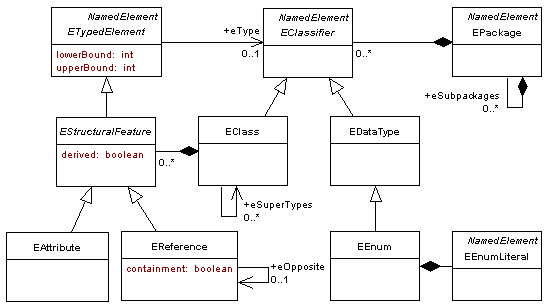
\includegraphics[width=\textwidth]{ecore.png}
\caption{Мета-мета-модель \tool{Ecore}}\label{Ecore}
\end{figure}

На \figref{Ecore} изображена диаграмма мета-мета-модели \tool{Ecore}. Согласно объектно-ориентированной парадигме, центральным понятием в \tool{Ecore} является класс. Экземпляры \tool{Ecore} (то есть мета-модели) представляют собой наборы классов, организованные в пакеты и связанные отношением ``общее-частное'', аналогичным наследованию в объектно-ориентированных языках программирования \cite{OOAD}. На \figref{ComponentClassEcore} показано, как элементы мета-модели, описывающей модели зависимостей между компонентами (такие как \figref{DiagramExample}) связаны с соответствующими мета-элементами в \tool{Ecore}.

//ComponentClassEcore

Следует обратить внимание на то, что \tool{Ecore} сама состоит из классов, что и позволяет ``оборвать'' иерархию мета-уровней, не используя $M^4$ (в действительности, иерархия не обрывается, просто все уровни, начиная с $M^3$ совпадают между собой и содержат только мета-мета-модель, то есть в нашем случае --- \tool{Ecore}).

В этом разделе мы опишем несколько основных концепций, используемых \tool{Ecore} (и другими мета-мета-моделями), которые будут использованы при изложении дальнейшего материала.

\paragraph*{Классы.} Как мы уже отмечали выше, основными элементами мета-моделей, описанных с помощью \tool{Ecore}, являются классы. Каждый класс имеет имя уникальное в пределах пакета, список суперклассов и список структурных элементов, атрибутов и ссылок. Экземпляры классов хранят значения для всех атрибутов и ссылок, объявленных самим классом и всеми его суперклассами (что соответствует наследованию членов классов в объектно-ориентированных языках). Класс может быть помечен как абстрактный. Такой класс не может иметь непосредственных экземпляров, экземпляры могут иметь только его подклассы, не являющиеся абстрактными.

Заметим, что понятие абстрактного класса в \tool{Ecore} является чисто номинальным, никаких технических препятствий к созданию экземпляра класса (таких как, например в \tool{Java} или \tool{C++}) быть не может, поскольку \tool{Ecore} не определяет тела методов. 

\paragraph*{Примитивные типы и перечисления.} Классы --- не единственное средство типизации в \tool{Ecore}, кроме них используются примитивные типы данных (Data Types) и перечисления (Enums). Примитивный тип данных представляет собой именованную сущность, семантика которой либо не фиксируется, либо определяется тем языком программирования, на котором реализовано моделируемое ПО (в случае \tool{Ecore} это \tool{Java}). 

\tool{Ecore} определяет несколько встроенных типов данных, таких как строки, целые и вещественные числа и т. д.

Перечисления --- это типы имеющие конечное множество значений (литералов).

\paragraph*{Структурные элементы классов: атрибуты и ссылки.} Основное отличие классов и примитивных типов данных --- в их назначении. Классы являются типами объектов, из которых состоят модели, а примитивные типы и перечисления --- типами значений атрибутов этих объектов. Таким образом, ссылки, определяемые классами могут иметь в качестве типа только класс, а атрибуты --- только примитивный тип или перечисление.

В остальном ссылки и атрибуты очень похожи. И те, и другие имеют имя и кратность, которая задается как пара чисел, определяющих нижнюю и верхнюю границу для количества значений, хранимых атрибутом или ссылкой. Так, например, ссылка \code{dependsOn} на \figref{DiagramExample} имеет кратность ``от 0 до $\infty$'', что означает, что компонента может зависеть от нуля или более других компонент. Атрибут \code{name} на том же рисунке имеет кратность ``от 1 до 1'', что означает, что каждая компонента должна иметь имя, причем ровно одно.

Как атрибуты, так и ссылки могут быть помечены как ``упорядоченные''. Этот флаг имеет значение для множественных ссылок и атрибутов (верхняя граница кратности которых больше единицы), и означает, что порядок объектов, на которые указывают ссылки (или значений атрибута) важен. Например, в классе \code{Block}, описывающего блок кода в программе и имеющего ссылку \code{statements}, указывающую на последовательность предложений внутри блока, ссылка \code{statements} должна быть упорядоченной, поскольку нам важно знать, в каком порядке выполнять предложения, из которых состоит блок.

\paragraph*{Перекрестные ссылки и агрегация.} Ссылки в \tool{Ecore} подразделяются на два вида: \term{перекрестные} и \term{агрегирующие}. Различие состоит в том, что на один объект не может быть более одной агрегирующей ссылки, то есть объект, имеющий агрегирующую ссылку, ``владеет'' объектом, на который ссылается. Для перекрестных ссылок таких ограничений нет, на любой объект может быть сколько угодно перекрестных ссылок.

Таким образом, если рассматривать модель как граф, ребрами в котором являются ссылки, то любой цикл обязан проходить хотя бы по одной перекрестной ссылке, а агрегирующие ссылки в модели определяют остовный лес \cite{cormen01introduction}.

Явное выделение агрегирующих ссылок позволяет легко представлять модели в древовидной форме, как показано на \figref{ModelTree}.

\begin{figure}[htbp]
\centering
%\includegraphics[width=\textwidth]{model_tree.jpg}
\caption{Представление модели в древовидной форме}\label{ModelTree}
\end{figure}

\paragraph*{Параметризованные типы.} Поскольку \tool{Ecore} развивается на платформе \tool{Java}, с выходом \tool{Java} 5 в мета-мета-модель были добавлены \term{обобщенные типы} (generic types, \cite{GJ}). Любой класс или тип данных может иметь параметры, которые могут служить типами для структурных элементов.

\section{Текстовая нотация для мета-моделей}
//


\chapter{Предметно-ориентированные языки}

Одновременно с мета-моделированием развивается концепция \term{предметно-ориентированных языков (ПОЯ)} (Domain-Specific Languages, DSLs \cite{StateMachine}). В рамках этой концепции утверждается, что во многих предметных областях существуют типичные задачи, для решения которых целесообразно разрабатывать специализированные языки, позволяющие легко выразить специфичные для данной области понятия. ПОЯ противопоставляются \term{языкам общего назначения} (General-Purpose Languages, GPLs), таким, например, как популярные языки программирования (\tool{C}, \tool{C++}, \tool{Java}, \tool{C\#} и т.д.). Задачи, специфичные для данной области, можно решать и с помощью языков общего назначения, но при таком подходе решения получаются гораздо большими по объему и содержат много однотипного кода, который не всегда возможно выделить в библиотеку. Кроме того, поскольку ПОЯ оперируют понятиями предметной области, они становятся более доступными для понимания экспертами в этой области, не имеющими навыков программирования, что облегчает процесс общения с заказчиком и позволяет снизить затраты.

В качестве примеров ПОЯ можно привести
\begin{enumerate}
\item издательскую систему \TeX ;
\item язык разметки \tool{HTML};
\item языки, используемые в конфигурационных файлах, например, для веб-сервера \tool{Apache};
\item язык для вывода графики \tool{PostScript};
\item язык описания графов \tool{GraphViz};
\item нотация EBNF для описания контекстно-свободных грамматик;
\item структурированный язык запросов для реляционных баз данных \tool{SQL};
\item и многие другие.
\end{enumerate}

Некоторые ПОЯ, например \TeX , являются универсальными в том смысле, что с их помощью можно описать любое вычисление, однако они спроектированы так, что с их помощью легко решать задачи в соответствующей предметной области, а описывать другие вычисления --- гораздо сложнее (как правило сложнее, чем на языках общего назначения).

\chapter{Понятие языка}

Несмотря на то, что концепции мета-моделирования и ПОЯ развивались независимо, они тесно связаны между собой, поскольку мета-модели логично рассматривать как языки описания моделей (а мета-мета-модель, соответственно, как язык описания мета-моделей). Таким образом, \tool{Ecore} (MOF, KM3 и т. д.) можно рассматривать как ПОЯ для описания ПОЯ. Эта точка зрения приобретает все большую популярность \cite{}.

Для более глубокого понимания взаимосвязей мета-моделирования и ПОЯ требуется определить само понятие ``язык''. В разных областях математики, логики и компьютерных наук это делается по-разному \cite{???}, например в математической логике термин ``язык'' часто используется как синоним термина ``множество''; нередко имеется в виду множество, описанное определенным образом \cite{}. Здесь и далее мы не будем говорить о языках ``вообще'', а ограничим наше рассмотрение \term{языками моделей}:

\newcommand{\Lang}[1]{\mathcal{L}\left(#1\right)}%
\newcommand{\LMM}[1]{\Lang{\MM{#1}}}%

\begin{Def}
Пусть задана мета-модель $\MM{M}$. Будем называть множество всех моделей, являющихся экземплярами $\MM{M}$, \term{языком, порожденным этой мета-моделью}, и обозначать $\Lang{\MM{M}}$.
\end{Def}

Это определение позволяет описывать как языка моделирования, такие как UML \cite{???}, которые изначально задаются с помощью мета-моделей, так и языки в более традиционном понимании. Например, в теории формальных языков \cite{???} принято определять язык как множество строк над конечным алфавитом; под наше определение подпадают те из языков, определенных таким образом, для которых есть конечное описание в виде (не обязательно контекстно-свободной) грамматики \cite{???}. Мета-модель, соответствующая грамматике состоит из классов, описывающих структуры термов соответствующей индуцированной алгебры \cite{???}.

\ignore{

Для того, чтобы рассуждать о большинстве языков, используемых на практике (например, о языках программирования), ниже мы определяем понятия, связанные с ``синтаксисом'' языков.

\section{Синтаксис}

Понятие ``синтаксис'', чаще всего ассоциируемое с правилами записи предложений языка, является сильно перегруженным и требует внимательного рассмотрения во избежание путаницы в терминах. В данном разделе мы постараемся разделить различные категории понятий, подразумеваемые в разных контекстах под словом ``синтаксис'', и ввести соответствующие определения.

\paragraph*{Конкретный синтаксис. } Способ визуального отображения языка мы будем называть \term{нотацией} (или \term{конкретным синтаксисом}) этого языка.

Для одного и того же множества языка $\LMM{M}$ можно задать несколько (бесконечно много) разных способов отображения. Среди всевозможных нотаций выделяют следующие практически важные классы:
\begin{enumerate}
\item текстовые нотации: предложения языка отображаются в виде строк символов некоторого конечного алфавита;
\item графические нотации: предложения языка отображаются в виде графических изображений, при этом роль играет цвет, форма и толщина линий, взаимное расположение объектов.
\end{enumerate}

Важной разновидностью текстового конкретного синтаксиса является ``расширяемый язык разметки'' (eXtensible Markup Language, XML \cite{XML}), являющийся на сегодняшний день промышленным стандартом для структурирования информации, хранимой в виде текста. Идейным предшественником XML можно считать нотацию S-выражений языка \tool{Lisp} \cite{LISP}.

Формально говоря, текстовый конкретный синтаксис можно считать разновидностью графического, но обычно такая классификация не представляет интереса, хотя в последние годы с появлением псевдо-текстового синтаксиса (системы MPS \cite{MPS}, Amadeus \cite{Amadeus}, SymADE \cite{SymADE}) граница между этими двумя понятиями постепенно стирается.

// Почему мы выбираем текстовый синтаксис? (Надо ли оно?)

Мы будем использовать следующее определение нотации:

\newcommand{\NNot}[3]{#1^{{#2} \rightarrow{} {#3}}}
\newcommand{\Not}[3]{\NNot{#1}{\MM{#2}}{\MM{#3}}}
\newcommand{\N}[2]{\Not{#1}{#1}{#2}}

\begin{Def}
\term{Нотацией} $\N{N}{M}$ для языка $\LMM{M}$ будем называть кортеж, состоящий из следующих объектов:
\begin{enumerate}
\item мета-модель $\MM{N}$;
\item однозначная вычислимая функция $$Meaning_N : \LMM{N} \rightarrow (\{\bot\} \cup \LMM{M}),$$ определенная везде на области задания.
\end{enumerate}

Там, где из контекста ясно, о каких мета-моделях идет речь, мы будем обозначать нотацию как $\Not{N}{}{}$.
\end{Def}

Согласно этому определению, нотация $\N{N}{M}$ задается некоторым множеством $\LMM{N}$ (в случае текстовых нотаций мета-модель $\MM{N}$ просто описывает произвольную последовательность символов, см. \figref{TextMM}), элементы которого преобразуются в элементы языка функцией $Meaning_N$ (в некотором смысле, эта функция выполняет роль, аналогичную роли компилятора языка программирования). Если функция $Meaning_N$ возвращает элемент $\bot$, это означает, что соответствующий элемент нотации некорректен (например, текст программы содержит синтаксическую ошибку).

\begin{figure}[htbp]
\caption{Мета-модель текста}\label{TextMM}
\end{figure}

Для одного и того же языка можно определить несколько нотаций, причем различные нотации не обязаны иметь различные мета-модели. Так, например, текстовых нотаций (заданных одной и той же мета-моделью \figref{TextMM}) для одного языка можно определить бесконечно много (например, добавляя обязательное ключевое слово в начало текста программы).

В широком смысле можно говорить о том, что нотация $\N{N}{M}$, точнее функция $Meaning_N$, определяет \term{денотационную семантику} \cite{???} языка $\LMM{N}$ в терминах языка $\LMM{M}$.

Всякий компилятор можно рассматривать как реализацию функции $Meaning_N$, где нотация $N$ является текстовой. Однако, как правило, компиляторы не работают ``в один шаг'', а выполняют серию преобразований из одной нотации в другую. Так, стандартной последовательностью является (1) преобразование текста в последовательность лексем, далее (2) построение абстрактного синтаксического дерева, которое (3) преобразуется во внутреннее представление, которое, после (4) оптимизации, (5) транслируется в машинный код \cite{Dragon}. Этот процесс можно рассматривать как одну трансформацию из текста в машинный код, а можно выделить в нем не менее пяти указанных этапов, имеющих, каждый, свои входной и выходной языки. Ниже мы часто будем прибегать к такому детализированному рассмотрению.
\newcommand{\Comp}[2]{#1 \circ #2}
\begin{Def}
Нотация $\N{N}{M}$ является \term{композицией} нотаций $\Not{A}{N}{B}$ и $\N{B}{M}$ и обозначается $\Comp{A}{B}$, если 
	$$Meaning_N(n) := \left\{\begin{array}{ll}
		Meaning_{A}(Meaning_{B}(n)), & \mbox{при } Meaning_{B}(n) \neq \bot\\
		\bot, & \mbox{в противном случае}
	\end{array}\right.$$
\end{Def}

Смысл условия в данном определении состоит в том, что если на некотором этапе была обнаружена ошибка ($\bot$), она не теряется, а распространяется на остальные этапы. Поскольку компиляторы следуют этой стратегии (не замалчивают ошибки), описанный выше процесс компиляции можно рассматривать как композицию пяти нотаций.

%На первый взгляд, согласно нашему определению, каждый новый способ отображения дает новый язык, однако такая интерпретация не неудобна с практической точки зрения: многие системы (Intentional \cite{Intentional}, MPS \cite{MPS}, GMF \cite{GMF} и др.) позволяют отображать одни и те же данные разными способами (этот подход называется \term{проективное редактирование}, Projection Editing \cite{Projection}), поэтому целесообразно говорить о том, что те или иные способы отображения относятся к одному и тому же языку (можно считать, что объединение нескольких видов конкретного синтаксиса само по себе является единым способом визуального отображения). 

\paragraph*{Абстрактный синтаксис. } Понятие ``абстрактного синтаксиса'' в литературе трактуется по-разному \cite{Dragon ...}, поскольку существует много различных ``уровней абстракции'' (по сути, различных нотаций, объединенных последовательной композицией).

Так, рассматривая языки с текстовым конкретным синтаксисом, под абстрактным синтаксисом чаще всего понимают алгебру термов, индуцированную грамматикой, описывающей конкретный синтаксис. В этом случае говорят об абстрактных синтаксических деревьях (Abstract Syntax Tree, AST), рассматривая их как деревья разбора, из которых удалены элементы, не представляющие интереса. Текст можно рассматривать как нотацию для языка таких термов, а соответствующую функцию $Meaning$ реализует синтаксический анализатор (обычно, в композиции с лексическим, но не всегда \cite{SGLR}).

Однако при рассмотрении языков с графическим или псевдо-текстовым конкретным синтаксисом  \cite{MPS, ...} под абстрактным синтаксисом понимают множество всех предложений языка, которое как правило явно задается некоторой мета-моделью (сами предложения являются моделями, то есть типизированными атрибутированными графами).

Следует отметить, что трансляторы текстовых языков обычно выполняют (явное или неявное) преобразование AST в граф, когда разрешают имена в программах (так имя переменной преобразуется в ссылку на объявление этой переменной). Таким образом, возникают понятия \term{первичного} абстрактного синтаксиса (First-Order Abstract Syntax, FOAS) и абстрактного синтаксиса \term{высшего порядка} (Higher-Order Abstract Syntax, HOAS). 

Чтобы избежать путаницы, мы будем придерживаться следующих обозначений:

\begin{Def}
Множество $\LMM{M}$ мы будем называть \term{содержанием} нотации $\N{N}{M}$. Мета-модель $\MM{M}$ будем называть \term{целевой мета-моделью} данной нотации.
\end{Def}

\begin{Def}
Понятие \term{абстрактного синтаксического дерева} (AST) имеет смысл только в связи с некоторой контекстно-свободной грамматикой. AST является термом соответствующей индуцированной алгебры, представленным в форме дерева объектов.
\end{Def}

\section{Графические и текстовые нотации}

Для ПОЯ чаще всего применяются...

\paragraph*{Использование графических нотаций при мета-моделировании}

Модели естественно отображать графически: деревья EMF, диаграммы UML

Очень наглядно, но большие диаграммы трудно читать и укладывать.
Для отображения нужны специальные довольно сложные инструменты.

\paragraph*{Преимущества текстового синтаксиса}

Работает даже в консоли. Независимость от инструментов, поддержка обобщенными инструментами (отображение, редактирование, сравнение, контроль версий). Это не работает для XMI из-за ссылок. появилась HUTN, но ей трудно пользоваться.

недостатки текста: надо парсить сложным алгоритмом, поддерживать параллельно структурное представление со ссылками и т.д.

\paragraph*{Псевдо-текстовый синтаксис}

MPS обладает всеми недостатками графического синтаксиса (редактировать и читать чуть проще, да)

\chapter{Ядро нотации и инфраструктурная функциональность}

Интуитивно понятно, что некоторая часть нотации может быть ``избыточной'' в том смысле, ее можно не использовать, сохраняя при этом возможность выразить все предложения языка, выразимые в исходной нотации. Примером таких избыточных элементов могут служить сокращенные формы записи для часто используемых конструкций языка\footnote{часто их называют ``синтаксическим сахаром'' (syntactic sugar \cite{???})}, такие как оператор \texttt{for} в языке \tool{C} \cite{???}, который легко можно выразить через другие операторы. В данном разделе мы вводим для описания таких элементов понятие \term{инфраструктуры} в рамках нотации, и показываем, что многие возможности в языках программирования, ориентированные на повторное использование, могут быть описаны как инфраструктурные.

\newcommand{\Infra}[1]{Infra\left(#1\right)}
\newcommand{\Core}[1]{Core\left(#1\right)}

\begin{Def}
\term{Множеством инфраструктурных элементов} нотации $\N{N}{M}$ называется максимальное по включению множество $\Infra{N}$ элементов мета-модели $\MM{N}$, исключение которого из рассмотрения не сужает образа функции $Meaning_N$:
	$$
		Meaning_N\left[
			\Lang{\MM{N} \setminus \Infra{N}}\right] = Meaning_N[\LMM{N}]
	$$
	
Множество элементов, не являющихся инфраструктурными, будем называть \term{ядром нотации} $N$ и обозначать $\Core{N}$.
\end{Def}

\begin{Def}
	Нотацию, для которой множество $\Infra{N}$ пусто, будем называть \term{минимальной}.
\end{Def}

\begin{Prop}
	Любую нотацию можно представить как композицию $\Comp{A}{B}$, где $B$ является минимальной нотацией.
\end{Prop}
\begin{proof}
Рассмотрим произвольную нотацию $\N{N}{M}$. Если она является минимальной, то она представима в виде
	$$\N{N}{M} = \Comp{\Not{1}{N}{N}}{\N{N}{M}},$$
где $\Not{1}{N}{N}$ --- \term{тождественная} нотация (имеет в качестве содержания самое себя).

Если $N$ не является минимальной, существует нотация $\NNot{\underline{N}}{\Core{N}}{\MM{M}}$, являющаяся минимальной частью $N$: ее можно получить, сузив функцию $Meaning_N$ на ядро нотации $N$. Для каждого предложения $m$ языка $\LMM{M}$ можно выбрать ``каноническое представление'' в нотации $\underline{N}$, то есть элемент $Norm(m) \in \Core{N}$, такой что $Meaning_{\underline{N}}(Norm(m)) = m$.

Теперь рассмотрим нотацию $\NNot{\overline{N}}{\MM{N}}{\Core{N}}$ с функцией
	$$Meaning_{\overline{N}}(n) := Norm(Meaning_N(n)),$$
легко видеть, что $N = \Comp{\overline{N}}{\underline{N}}$.
\end{proof}

Мы показали, что инфраструктурная функциональность может быть выражена статически как трансляция расширенной нотации в минимальную.  Ниже мы покажем, что многие возможности языков программирования, связанные с повторным использованием, могут быть выражены с использованием только инфраструктурных элементов. Это позволяет реализовывать такие возможности отдельно от основных возможностей языка, а также автоматизировать их создание.

Повторное использование всегда базируется на тех или иных механизмах композиции: средствах, позволяющих комбинировать одни и те же объекты многими способами.

// Пояснить

??? В принципе, композиция может поддерживаться не только на уровне инфраструктуры, но и на уровне содержания языка. Например, как мы покажем ниже, модули часто являются элементами инфраструктуры, а функции и классы, также обеспечивающие композицию, имеют динамическую семантику и, следовательно, являются неотъемлемыми элементами содержания языка.

??? Рассмотрим наиболее широко используемые средства композиции, которые как правило обеспечиваются инфраструктурой.

\section{Механизмы идентификации}

Для реализации механизмов повторного использования (композиции) необходимо, чтобы в языке была возможность \term{идентификации} внутри программы, то есть, чтобы из одной части программы можно было сослаться на элемент, определенный в другой ее части. Чаще всего для этой цели используются имена --- уникальные строковые идентификаторы присваиваемые переменным, функциям и т. д., однако нередко используются и более сложные механизмы, например квалифицированные имена (пакет + подпакеты + класс) в \tool{Java} \cite{JLS} или сигнатуры функций при перегрузке в \tool{C++} \cite{???}. Так или иначе, элементам программы сопоставляются \term{идентификаторы} --- объекты, уникальные в определенной области видимости. Важно отметить, что идентификатор не обязан быть уникальным глобально: во-первых, если он уникален в рамках поименованной области видимости, которая, в свою очередь, имеет глобальный идентификатор, этой информации достаточно, чтобы глобально идентифицировать объект; в этом случае мы будем говорить о составном идентификаторе, включающем идентификатор области видимости. Во-вторых, идентифицируемый объект может быть принципиально не доступен из некоторых областей видимости, как, например, локальная переменная, которая ``не существует'' за пределами функции, в которой она объявлена. К таким объектам не должно быть доступа извне, а следовательно и глобальных идентификаторов.

%Наша задача --- показать, что идентификаторы как таковые в большинстве языков являются инфраструктурными элементами нотации. Интуитивно, аргументом в пользу этого является тот факт, что при согласованном переименовании всех упоминаний некоторого элемента в программе, смысл программы (то есть значение функции $Meaning_N$) остается прежним\footnote{Исключением из этого правила являются языки с динамическими возможностями, в частности, поддерживающие \term{рефлексию} \cite{???}.}. В теории функционального программирования такое преобразование называется $\alpha$-редукцией \cite{???}; в силу значительных неудобств, связанных с формализацией $\alpha$-редукции при описании семантики различных $\lambda$-исчислений, были разработаны методы, позволяющие полностью избавиться от имен при описании семантики \cite{HOAS, NomL}.

Пусть $\MM{C}$ --- мета-модель, описывающая машинный код (или язык ассемблера) некоторого процессора или виртуальной машины. Язык $L$, компилируемый для этого процессора или виртуальной машины, можно рассматривать как нотацию $\N{L}{C}$. Эту нотацию можно представить как композицию двух других нотаций: 
$$N{L}{C} := \Comp{\Not{P}{L}{G}}{\Not{Q}{G}{C}},$$
причем в мета-модели 
Ссылки на переменные (вложенные области видимости)
Ссылки на функции и перегрузка
Пространства имен (могут быть и вложенными)
Атрибуты доступа?

\section{Модули}

В большинстве языков программирования \term{модулями} называются фрагменты программ, пригодные для повторного использования путем цитирования: при необходимости обратиться к коду, находящемуся внутри модуля, достаточно ``подключить'' этот модуль в текущей области видимости, после чего можно пользоваться именованными элементами программы, определенными в этом модуле. \cite{???}

Цитирование является, очевидно, простейшим из возможных способов композиции --- одна часть программы просто ссылается на другую. Рассмотрим механизмы работы модулей в различных языках программирования и возможности реализации этих механизмов как инфраструктурных элементов нотации. Нотацию каждого языка мы попытаемся разделить на ядро и инфраструктуру, таким образом, чтобы все, что касается модулей, оказалось в инфраструктурной части.

\paragraph*{Язык \tool{C}. } Вероятно, самая простая реализация модулей принята в языке программирования \tool{C} \cite{???}. Строго говоря, в языке \tool{C} модули вообще не поддерживаются, поскольку обработкой подключаемых заголовков занимается отдельная программа --- \term{препроцессор} \cite{???}, которая способна обрабатывать произвольный текст, размеченный специальными \term{директивами}, а не только код, написанный на языке \tool{C}. 
Однако, поскольку спецификация препроцессора включена в стандарт, и практически никакая программа на \tool{C} не мыслима без его использования, мы будем рассматривать директивы препроцессора как часть нотации языка \tool{C}.

Объявления библиотечных функций и структур данных делаются в отдельных файлах, называемых \term{заголовочными} (header files). Эти файлы, как правило, не содержат реализаций функций, которые помещаются в \term{исходных файлах} (source files). Исходные и заголовочные файлы могут использовать директивы включения \code{\#include}. Препроцессор, обрабатывает исходные файлы по отдельности, вставляя текст включаемых файлов вместо директив включения, пока в тексте есть такие директивы. Таким образом, в результате получается один файл, содержащий все прямо или косвенно включенные объявления, который, в свою очередь, обрабатывается компилятором.

Из сказанного выше видно, что процесс обработки исходного текста включает фазу, которая переводит программу в более богатой нотации (с директивами включения) в программу в менее богатой нотации. Поэтому мы можем рассматривать директивы препроцессора как инфраструктурную часть нотации языка \tool{C}, а отделение препроцессора от компилятора --- как декомпозицию нотаций. 

Вывод: в языке \tool{C} механизм композиции обеспечивается с помощью инфраструктурных элементов нотации. 

\paragraph*{Язык \tool{Pascal}. } В языке \tool{Pascal} \cite{???} модули (units) являются частью основной нотации: каждый модуль имеет имя, которое используется для ссылок на него (в отличие от имени файла в случае \tool{C}), объявления, сделанные в модуле получают идентификаторы в соответствующем пространстве имен, то есть если имена функций, объявленных в разных модулях, совпадают, у программиста есть возможность явно указать, об объявлении из какого модуля идет речь в программе. Сходство с \tool{C} заключается в том, что каждый модуль определяется в отдельном файле, имеется способ подключения модулей, в модуле выделяется интерфейсная часть, в которой, как и в заголовочном файле в \tool{C}, могут содержаться только объявления. Можно сказать, что система модулей \tool{Pascal} гораздо больше контролируется статически, в отличие от \tool{C} (это утверждение верно и при сравнении другой функциональности этих языков). 

Несмотря на то, что в случае языка \tool{Pascal} механизм, обрабатывающий модули, интегрирован в компилятор и не является отдельной программой как препроцессор \tool{C}, мы можем представить нотацию этого языка как композицию двух нотаций, вторая из которых не содержит модулей (то есть реализовать модули как инфраструктурную часть нотации). Функцию $Meaning$ для первой нотации достаточно реализовать аналогично принципу работы препроцессора в \tool{C}: вставить текст модулей в использующие из программы (переименовывая элементы в случае повторений \cite{capture-avoiding-substitution})\footnote{В некоторых случаях будет необходимо добавить предварительные декларации для типов и функций, но это всегда возможно сделать, поскольку \tool{Pascal} запрещает циклические зависимости между интерфейсами модулей}. Программа, полученная в результате не будет содержать следующих элементов: предложений \code{uses} (включений модулей), объявлений модулей (\code{unit interface ... implementation ... end}), имен переменных, функций и типов, квалифицированных именами модулей для разрешения конфликтов (эти элементы будут переименованы).

Вывод: механизм модулей языка \tool{Pascal} можно представить в виде инфраструктурной части нотации.

\paragraph*{Язык \tool{Java}.} Модули, аналогичные тем, что есть в \tool{Pascal} и \tool{C}, в языке \tool{Java} в чистом виде не представлены: функции пространств имен для объявлений выполняют классы, которые также являются объявлениями типов \cite{JLS}. Наиболее близким к традиционным модулям понятием в \tool{Java} является \term{пакет} (package) --- пространство имен, в котором объявляются только типы (классы, интерфейсы, перечисления). Пакеты с модулями роднит в первую очередь механизм \term{импортирования}: чтобы воспользоваться типом, объявленным в другом пакете, программисту необходимо написать предложение \code{import} или квалифицировать имя класса именем пакета.

Если не принимать во внимание динамических возможностей языка \tool{Java} (в первую очередь, библиотеки \code{reflection}, позволяющей обращаться к классам и методам по идентификаторам, записанным в виде строк \cite{JLS}), пакеты можно выразить как инфраструктурную функциональность (аналогично модулям в \tool{Pascal}). Но этот подход воспрепятствует правильной работе механизмов, основанных на динамической загрузке классов, таких, например, как использование одного экземпляра библиотеки несколькими приложениями.

Вывод: механизм пакетов языка \tool{Java} можно выразить с помощью инфраструктуры нотации лишь частично.

\section{Шаблоны}

В предыдущем разделе мы видели, в какой мере модули могут быть выражены как инфраструктура нотации. Общий вывод таков: статическая композиция выражается легко, а динамическая --- не выражается. Это вполне естественно, поскольку само понятие инфраструктуры нотации основывается на \emph{статической} композиции, а не на динамической. Грубо говоря, инфраструктура описывает часть программы, которая может быть полностью вычислена во время компиляции.

Модули представляют собой самый простой механизм композиции. В данном разделе мы рассмотрим механизм \term{макроопределений} (или ``шаблонов''), который, не котором смысле обобщает механизм модулей и предоставляет возможности для более гибкого повторного использования.

\paragraph*{Происхождение термина ``шаблон''.} Термин ``шаблон'' (template) позаимствован из языка программирования \tool{C++} \cite{???}. Этот язык позволяет программисту определять не только классы и функции, но и шаблоны классов и функций --- параметризованные определения, которые можно \term{инстанцировать}, указав значения параметров. Как правило, параметрами являются типы, но можно использовать и константы. Изначально шаблоны были введены в язык для того, чтобы поддержать параметрический полиморфизм \cite{???}, который необходим для реализации удобной библиотеки контейнеров \cite{???}, однако оказалось, что шаблоны позволяют сделать гораздо больше \cite{???}, например, и их помощью можно вычислить во время компиляции любую рекурсивную функцию \cite{???}, то есть компилятор \tool{C++} представляет собой интерпретатор вычислительно универсального языка, основными элементами которого являются шаблоны.

Так или иначе, шаблоны являются частью инфраструктуры нотации языка, поскольку на этапе компиляции каждое упоминание шаблона разворачивается в результате подстановки аргументов на место параметров, и становится обыкновенной функцией или классом. Здесь необходимо заметить, что вследствие вычислительной универсальности шаблонов, процесс их разворачивания может никогда не закончиться (можно написать ``программу'' на шаблонах, порождающую бесконечную цепь рекурсивных обращений шаблонов к самим себе), этот сценарий мы будем считать ошибкой компиляции, то есть функция $Meaning$ для такого входа возвращает $\bot$.

// Haskell \textbf{Template} Meta-programming

\paragraph*{Происхождение термина ``макроопределение''.} Термин ``макроопределение'' (macro-definition или macro\footnote{В некоторых русскоязычных источниках можно встретить слово ``макрос'' (как единственное число существительного мужского рода в именительном падеже), которое образовано транслитерацией слова ``macros'', являющегося формой множественного числа. В силу его грамматической несогласованности, мы избегаем использования этого термина.}) восходит к языкам семейства \tool{Lisp} \cite{???}. Так называется определение в программе, часто --- параметризованное, на которое можно сослаться по имени как на функцию, но оно будет заменено в тексте программы до его выполнения. Например, в языке, где параметры функциям передаются по значению, повторно используемую подпрограмму для обмена переменных местами можно реализовать в виде макроопределения \cite{???}.

\begin{lstlisting}[language=Lisp,label=scheme_swap]
 (define-syntax-rule (swap x y)
    (let ([tmp x])
      (set! x y)
      (set! y tmp)))
\end{lstlisting}

Обращение к этому определению будет заменено на фрагмент программы, меняющий местами значения двух переменных, тогда как вызов функции менял бы местами значения их локальных копий в стеке.

Макроопределения (как и шаблоны) часто используются для создания встроенных предметно-ориентированных языков \cite{???}, поскольку они позволяют в некотором смысле расширить язык программирования новыми конструкциями (то есть, в каком-то смысле, добавить в нотацию новые инфраструктурные элементы).

Очевидны сходства макроопределений \tool{Lisp} с шаблонами \tool{C++}: и те, и другие являются параметризованными фрагментами программ, которые разворачиваются во время компиляции. 

\paragraph*{Обработка идентификаторов при разворачивании макроопределений и шаблонов.}
Разворачивание макроопределений (и шаблонов) связано с проблемой повторения идентификаторов. Если обратиться к макроопределению, меняющему местами значение двух переменных через переменную \code{tmp}, дважды, имя \code{tmp} будет объявлено дважды, что во многих языках вызовет ошибку. В других языках это может привести к изменению значения другой переменной, имя которой случайно совпало с \code{tmp}.

В некоторых системах (как, например, в упоминавшемся выше препроцессоре языка \tool{C}, поддерживающем также и макроопределения) решение этих проблем полностью возлагается на программиста: его внимательность и осторожность. Более совершенные системы гарантируют обнаружение подобных ошибок во время компиляции.

В случае шаблонов \tool{C++} задача относительно проста, поскольку тело шаблона (функция или класс) является пространством имен, поэтому необходимо лишь отслеживать отсутствие повторений в именах шаблонов, а также обеспечить различение результатов развертывания с различными параметрами. Так, компилятор считает использования одного и того же шаблона класса \code{std::vector<int>} и \code{std::vector<string>} разными типами, несмотря на то, что имя шаблона повторяется. Таким образом, идентификатором результата развертывания является имя шаблона и его аргументы. При многократном упоминании одного и того же идентификатора (например, \code{std::vector<string>}) шаблон разворачивается только один раз. Можно говорить о том, что в \tool{C++} проблема именования при развертывании шаблона решена \emph{ad hoc}, за счет ограничения набора элементов, которые могут быть результатом развертывания.

В \tool{Lisp}\footnote{Речь идет о семействе \tool{Lisp} 2 \cite{???}} эта проблема решается в более общем виде: с помощью \term{генерирования свежих имен} и \term{гигиены}. Генерирование свежих имен реализовано специальной операцией \code{gensym}, которая порождает имя, не занятое в текущей области видимости. ``Гигиеной'' (hygiene) называется система средств, позволяющих во время развертывания макроопределения проверять, определено ли уже то или иное имя, и переименовывать элементы в случае необходимости.

// Подробнее



Те же модули, но с параметрами (полиморфные или обобщенные)
	то есть включение, но с внедрением пользовательской информации. Контроль на стороне клиента
	LISP
	макросы в C
	С++
	m4/ST/Vel
	Haskell Template Meta-programming
	Nemerle
	Macros as MultiStage Computations: TypeSafe,Generative, Binding Macros in MacroML
}	
\section{Аспекты}

Если смотреть на модули и шаблоны (макроопределения) как на механизмы композиции, они являются последовательными этапами на пути придания гибкости процессу комбинации фрагментов программы. Пусть есть два фрагмента: M (от Main, основная программа) и L (jn Library, библиотека), и M должен использовать часть функциональности L. В этом случае, при использовании простых модулей, M должен выбрать фрагменты L, которые ему нужны, и использовать их. В случае шаблонов, M не только выбирает нужные ему фрагменты, но и может модифицировать их, подставляя собственные значения шаблонным параметрам. Сказанное иллюстрируется \figref{Composition}.

\begin{figure}[htbp]
// Картинка: кружочек, кружочек с дырками, подписано, что L, а что M
\caption{Виды композиции}\label{Composition}
\end{figure}

Развитие этой линии приводит нас к следующему механизму композиции: M вообще не обязан выбирать сам, L может самостоятельно определить, каким частям программы понадобятся те или иные элементы. Такой механизм является дополнительным к описанным выше; он лежит в основе \term{аспектно-ориентированного программирования} (АОП, \cite{???}).

\paragraph*{Язык \tool{AspectJ}.} АОП получило распространение благодаря языку \tool{AspectJ} \cite{???}, созданному на основе \tool{Java}, добавляя конструкции для нового способа композиции (сразу видно, что речь во многом идет об инфраструктурной функциональности). Основными концепциями в новом языке стали \term{точки присоединения} (join points), \term{срезы} (point-cuts) и \term{советы} (advice). Все эти элементы определяются внутри структурных элементов, называемых \term{аспектами}. Аспекты определяют в себе черты классов, объединяющих взаимосвязанные функции и данные, и модулей, хранящих независимые элементы, одновременно.

Аспектно-ориентированная композиция заключается в том, что код \term{совета} встраивается в основную программу. Например, для записи информации о ходе выполнения в журнал, требуется вписать однотипный код во множество мест в программе. Аспекты позволяют решить эту задачу, написав необходимый фрагмент кода только один раз.

Позиции, в которые код может встраиваться, называются \term{точками присоединения}. В \tool{AspectJ} это позиции перед и после вызовов функций, присваиваний, создания объектов и т. д. Для того, чтобы присоединить \term{совет} сразу ко множеству точек, это множество задается с помощью выражений, называемых \term{срезами}. Срезы описывают статическое или динамическое положение точки в программе, например ``вызов метода a()'' или ``создание объекта класса, имя которого начинается на A, которое происходит в потоке управления метода x()''. При присоединении \term{совета} к срезу указывается относительное положение: \term{совет} может присоединяться \term{до} (before), \term{после} (after) или \term{вместо} (around) каждой точки присоединения, соответствующей срезу.

Частным случаем такого подхода является добавление аспектом полей и методов в существующие классы, причем исходный код самих этих классов не изменяется. Этот механизм носит название ITD (Inter-Type Declarations). Например, специальный аспект может реализовывать методы \code{toString} для нескольких классов в одном файле, объединяя таким образом эту функциональность в одном модуле:

\begin{lstlisting}[language={[AspectJ]Java}]
aspect ToString {
	public String A.toString() {
		return "A: " + data;
	}

	public String B.toString() {
		return "B: " + data;
	}

	public String C.toString() {
		return "B: " + data + " " + moreData;
	}
}
\end{lstlisting}

\paragraph*{Характеристические свойства АОП.} С момента появления языка \tool{AspectJ} разработано множество концепций, так или иначе ``напоминающих'' идеи, заложенные в этом языке. В 2000 году в работе \cite{Obliviousness} была предпринята попытка выработать определение АОП, чтобы иметь эффективный критерий, позволяющий сказать, является ли данный язык аспектно-ориентированным. Название работы говорит само за себя: ``Aspect-oriented programming is quantification and obliviousness''\footnote{\textit{(англ.)} Аспектно-ориентированное программирование --- это квантификация и незнание.}
Под \term{квантификацией} (quantification) понимается возможность охарактеризовать множество точек присоединения предикатом, записанном на специальном языке. Под \term{незнанием} (obliviousness) подразумевается, что программа, в которою встраиваются \term{советы}, не знает о том, что они есть, то есть никак не зависит от их кода (код советов может зависеть от кода этой программы).

Таким образом, можно говорить о том, что аспекты --- это ``шаблоны наоборот'': не M использует L, дополняя ее своими фрагментами, а L ``сама'' встраивается в M.

\paragraph*{Аспекты как инфраструктурная функциональность.} \tool{AspectJ} статически компилируется в байт-код платформы \tool{Java}\footnote{Это не единственный способ присоединения аспектов к \tool{Java}-программам. Кроме него поддерживается \term{динамическое встраивание}, при котором байт-код модифицируется при загрузке классов во время выполнения}, из которого можно однозначно восстановить исходный код Java-программы. Это преобразование можно представить как трансформацию кода \tool{AspectJ} в код на \tool{Java} с последующей компиляцией. То есть аспекты можно реализовать как элемент инфраструктуры нотации \tool{AspectJ}.

// Не сказать ли про другие языки?


Сложные правила композиции (взаимопроникающие модули, инвазивная композиция): внедрение доп. информации без ведома клиента (слабее зависимости), прозрачность и т.д.
	
	AspectJ, терминология
	АПОЯ
		примеры для разных доменов
		примеры для грамматик


\section{Распространение рассмотренных механизмов композиции}

табличка: что где есть

мы рассмотрели вот эти языки. эти фичи есть почти везде, значит их приходится часто реализовывать, значит это надо автоматизировать.

\section{Диалекты}

// Рассказать про задачу разработки диалектов трех типов
// Сослаться на статьи про эволюцию языков


%\chapter{Инструменты для автоматизации разработки текстовых языков}

В данном разделе мы рассматриваем существующие инструменты, автоматизирующие разработку языков. В основном, эти инструменты ориентированы на разработку предметно-ориентированных языков, поскольку такие языки необходимо разрабатывать часто, что делает затраты на реализацию даже элементарных возможностей таких языков часто повторяющимися, в результате чего возникает необходимость в максимальном сокращении таких затрат.

В первую очередь нас интересует, насколько существующие подходы позволяют автоматизировать поддержку механизмов композиции, описанных выше, однако мы будем также отмечать и другие особенности этих подходов, в частности, поддержку механизмов композиции в языках, используемых самими инструментами.

\ignore{
\section{Контекстно-свободные грамматики}

--- Описание грамматик
	BNF
	EBNF (шаблоны)
	
	КСГ
	продукция 
	правило 
	правая часть 
	символ 
	терминал 
	нетерминал

	индуцированная алгебра термов
	частичный тип

\section{Атрибутная трансляция}

определения
JustAdd, ITD в нем

	атрибут
	семантическое действие

\section{Синтаксически-управляемая трансляция}

недостаток АТ

определение СУТ, L-атрибутные определения

Генераторы на основе СУТ
	Yacc/Bison и компания
		LALR, только синтез. аттр
	ANTLR
		LL, и те, и те
		
	внедренные семантические действия
}				
\section{Внутренние ПОЯ}

Часто ПОЯ разделяют на \term{внешние} (external) и \term{внутренние} (internal) \cite{StateMachine}. Внешними называют языки, имеющие специальные средства обработки, например, транслятор, написанные именно для данного ПОЯ. Внутренние языки, напротив, не имеют специальных средств обработки: они ``встраиваются'' в языки общего назначения, как библиотеки или расширения другого рода. В принципе, любой прикладной программный интерфейс (Application Programing Interface, API) можно рассматривать как внутренний ПОЯ: функции API выполняют роль ``ключевых слов'' внутреннего языка. Как правило, о внутренних языках говорят, если соответствующий язык общего назначения позволяет обращаться к библиотекам, используя достаточно гибкие синтаксические конструкции.

// Пример про fluent interfaces

Популярными языками для встраивания ПОЯ являются, например, \tool{Groovy} \cite{Groovy}, \tool{Haskell} \cite{Haskell98}, \tool{Scala} \cite{Odersky2008} и \tool{Java} \cite{JLS}. Существуют языки, имеющие специальные механизмы для расширения синтаксиса, позволяющие очень удобно интегрировать внутренние языки, например, \tool{Nemerle} \cite{Nemerle} и \tool{PLOT} \cite{PLOT}.
		
\section{Модульность грамматических определений}

Как ни странно, далеко не все популярные инструменты поддерживают повторное использование грамматических определений, например, \tool{Bison} \cite{BisonBook}, \tool{CoCo/R} \cite{CocoR} и \tool{JavaCC} \cite{JavaCC} не поддерживают никаких механизмов такого рода. Это связано в первую очередь с тем, что грамматические определения ``двумерны'': они содержат как описание синтаксической структуры (продукции КСГ), так и описание вычислений (семантические действия), что затрудняет композицию. Кроме того, специальные классы грамматик (например, $LL(k)$) не замкнуты относительно объединения, что накладывает дополнительные трудности на композицию \cite{???}. Так или иначе, инженерная дисциплина при разработке трансляторов находится на гораздо более низком уровне, чем при разработке других видов ПО \cite{Grammarware}.

В данном разделе мы рассмотрим механизмы повторного использования грамматических определений, основанные на цитировании, то есть модули и шаблоны. Аспектно-ориентированная композиция грамматик рассматривается в следующем разделе.

\subsection{Модули и ограничение видимости} В работе \cite{SysProg-2006} приведен обзор наиболее популярных средств для разработки трансляторов и выполнено сравнение по нескольким критериям, одним из которых является повторное использование.

Простейшая реализация модулей представлена в инструментах \tool{Elkhound} \cite{Elkhound} и \tool{ANTLR} версии 3 \cite{ANTLR}, который поддерживает директиву \code{include} для подключения определение из других файлов. 

Несколько иной подход использован в генераторе \tool{Menhir} \cite{Menhir}, который, принимая на вход несколько файлов, просто ``склеивает'' их содержимое вместе, но позволяет контролировать, какие символы являются открытыми (public) и могут быть использованы в других файлах, а какие --- нет. Закрытые (private) символы автоматически переименовываются для того, чтобы избежать коллизий. Особенность идеи ``склеивания'' файлов состоит в отсутствии директивы цитирования (\code{include} или \code{import}), что облегчает реализацию механизма, но делает зависимости между модулями \emph{невидимыми}: читая отдельный файл, трудно понять, какие из упоминаемых символов определены в других модулях, а главное --- нет никакой возможности определить, в каких именно модулях они определены.

Более традиционным образом модули организованы в системе \tool{ASF+SDF} \cite{ASF+SDF}: аналогично подходу, принятому в языках программирования, каждый модуль имеет имя, соответствующее имени файла, в котором он определен, элементы, объявленные в модуле, делятся на открытые (\code{exports}) и закрытые (\code{hidden}), причем другие модули могут использовать только открытые элементы, что обеспечивает инкапсуляцию. Директива цитирования \code{import} позволяет подключать модули друг к другу. При импортировании может оказаться, что символ, объявленный в одном модуле имеет то же имя, что и символ объявленный в другом. Как мы видели выше, в некоторых языках эта проблема решается с помощью квалифицированных имен (среди инструментов разработки трансляторов такого подхода придерживается \tool{Rats!} \cite{Rats!}); в \tool{ASF+SDF} используется другой подход: директива цитирования позволяет при необходимости \term{переименовать} символ, импортируемый из данного модуля, например:

\begin{lstlisting}
module example/Example

imports library/Lib[ A => B ]
\end{lstlisting}

Теперь внутри модуля \code{example/Example} символ \code{A}, определенный в \code{library/Lib} будет иметь имя \code{B}.

\subsection{Наследование в грамматических определениях}
% Compiler generation based on grammar inheritance
Идея \term{наследования грамматик} была впервые предложена в работе \cite{GInh}, и основывается на том, что грамматика может наследоваться от другой грамматики, добавляя новые правила и переопределяя старые. Первоначальная реализация была выполнена на языке \tool{Smalltalk} для рабочей станции \tool{Sun 3}, и не получила широкого распространения, однако в дальнейшем наследование грамматик было реализовано в других инструментах.

В \tool{ANTLR} версии 2 \cite{ParrQ95} наследование грамматик является единственным механизмом их повторного использования. Грамматика может быть унаследована от не более, чем одной родительской грамматики, при этом возможно переопределение правил, а именно: изменение семантических действий (при сохранении синтаксической структуры),  добавление новых альтернатив к существующим правилам. Кроме переопределения, также можно определять и совершенно новые правила (которые могут ссылаться на символы, определенные в родительской грамматике). К недостаткам такого подхода к повторному использованию можно отнести тот факт, что наследование является одиночным, и у разработчика нет возможности использовать несколько независимых модулей при разработке одного языка. Создатели \tool{ANTLR} 2 в качестве основного сценария использования наследования грамматик указывали создание нескольких диалектов одного языка \cite{???}.
% http://www.antlr2.org/doc/inheritance.html

Множественное наследование атрибутных грамматик предложено в работе \cite{MAGInh} и реализовано в инструменте \tool{LISA}. %http://portal.acm.org/citation.cfm?id=606666.606678
Авторы уделили больше внимание повторному использованию семантических действий, но и синтаксическая структура может быть унаследована, дополнена и частично переопределена.
Важным дополнением к наследованию грамматик в \tool{LISA} являются \term{шаблоны}.

В некоторых объектно-ориентированных языках (таких, например, как \tool{Scala} \cite{Odersky2008}) альтернативой наследованию является ``подмешивание'' (mixins). Похожий механизм для грамматик реализует инструмент \tool{xText} \cite{xText}. Результирующий механизм близок к множественному наследованию грамматик, но более строго и просто определяет поведение системы в случае ``ромбовидного наследования'' \cite{C++}. Mixin в \tool{xText} может добавлять новые правила или продукции, а также переопределять существующие.

Единственным известным нам инструментом, позволяющим не только добавлять, но и удалять продукции, является \tool{Rats!} \cite{Rats!}. Этот инструмент не используем явным образом метафору наследования для грамматик: авторы говорят лишь о ``модификации импортируемых модулей'', однако функциональность, реализованная этой операцией схожа с тем, что в других инструментах достигается с помощью наследования грамматик: есть возможность добавить продукцию, заменить или даже удалить ее.


\paragraph*{Параметризованные определения (шаблоны).}
Идею использования шаблонов (макроопределений для продукций или правил) при описании формальных грамматик легко проиллюстрировать на следующем примере: в синтаксисе языков программирования очень часто встречаются списки --- последовательности элементов (например, имен переменных), разделенных специальным символом (например, запятой). Элементы и разделители разнятся в зависимости от контекста. В грамматике языка \tool{Java} \cite{JLS} такие конструкции встречаются не менее 14 раз. Для того, чтобы решить проблему списков однажды и навсегда, можно определить следующий шаблон:

\begin{lstlisting}
	list<item, sep> -> item (sep item)*;
\end{lstlisting}

В результате возникает возможность коротко описывать такие разные языковые конструкции как вызов функции и арифметическое выражение:

\begin{lstlisting}
	functionCall -> NAME '(' list<expression, ','> ')';
	arithExpr -> list<product, plusOrMinus>;
\end{lstlisting}

Действительно, в скобках при вызове функции указывается список выражений, разделенных запятыми, а арифметическое выражение --- это алгебраическая сумма произведений, то есть список произведений, разделенных плюсами или минусами.

Стандартизированная нотация EBNF \cite{EBNF} имеет поддержку таких несложных шаблонов, хотя большинство инструментов реализует шаблоны по-своему. Прообразом грамматик с шаблонами можно считать двухуровневые грамматики \cite{???} использованные при описании \tool{Algol68} \cite{Algol68}, однако они не получили широкого распространения: идея была упрощена и приспособлена для понимания инженерами.

Реализация шаблонов в \tool{Menhir} наиболее близка к требованиям стандарта EBNF: индивидуальные правила могут иметь параметры, которым сопоставляются значения при использовании. В \tool{LISA} поддерживаются шаблоны для семантических действий: параметрами являются вхождения атрибутов.

Еще один способ использования шаблонов при описании грамматик состоит в определении не отдельных правил или продукций с параметрами, а в параметризации целой грамматики. Этот подход может служить хорошей альтернативой наследованию грамматик (он, фактически, аналогичен \term{делегированию} в объектно-ориентированных языках \cite{Gamma1995}). Например, грамматика, определяющая арифметические выражения, может принимать синтаксическую форму для атомарных выражений в виде параметра:

\begin{lstlisting}
grammar template Arith<atom> {
	sum    -> mult (('+' | '-') mult)*;
	mult   -> factor ('*' factor)*;
	factor -> '(' sum ')';
	       -> <atom>;
}
\end{lstlisting}

Этот шаблон позволяет порождать грамматики для арифметических выражений над разными (атомарными) объектами, например, над целочисленными константами и переменными:

\begin{lstlisting}
grammar Arith<INT | VAR>;

INT -> [0-9]+;
VAR -> [a-zA-Z_][a-zA-Z_0-9]*;
\end{lstlisting}

Или над комплексными константами:

\begin{lstlisting}
grammar Arith<complex>;

complex -> '(' FLOAT ',' FLOAT ')';
FLOAT   -> INT '.' INT;
\end{lstlisting}

Параметризацию модулей поддерживают инструменты \tool{ASF+SDF} и \tool{Rats!}, но эти возможности реализованы в них по-разному. \tool{Rats!} позволяет использовать в качестве параметров только модули целиком: параметризованный модуль может импортировать модуль-параметр и обращаться к символам внутри этого модуля. Такой подход в наибольшей степени схож с идеей делегирования в ООП: модуль рассматривается как класс, а набор имен символов --- как интерфейс\footnote{Здесь правомерно говорить об аналогии со ``статическим полиморфизмом'' в \tool{C++} \cite{C++}.}. В \tool{ASF+SDF}, напротив, модуль не может быть параметром, в качестве таковых используются только отдельные символы. 

Оба подхода имеют свои недостатки: в \tool{Rats!}, чтобы передать всего один символ в качестве параметра, придется создать модуль, а в \tool{ASF+SDF} неудобно передавать много символов за один раз. Кроме того, шаблоны отдельных правил и выражений в этих инструментах создавать нельзя. Нам не известно о существовании инструмента, поддерживающего все три способа параметризации.
	
\section{Аспектно-ориентированные грамматические определения}

Следующим шагом в развитии средств повторного использования грамматических определений является поддержка аспектов.

// Переписать рассуждения про то, откуда croscutting concerns в грамматиках
// Добавить объяснения про то, что grammar duplication и entanglement при генерации специфических тулов

% Separation of concerns in compiler development using aspect-orientation --- 2006
В работе \cite{Wu06} отмечается, что даже использование аспектно-ориентированного языка общего назначения (\tool{AspectJ}) облегчает разработку трансляторов. Многие инструменты интегрировали поддержку аспектов с более традиционной функциональностью, описанной выше.

Широкую известность получил подход, использованный в системе \tool{JastAdd} \cite{JastAdd}, основанной на расширенном определении атрибутных грамматик. В рамках этого подхода (использованного также и в других работах, см. \cite{Silver}) типы вершин AST рассматриваются как классы, а атрибуты определяются как методы с помощью механизма ITD.

Системы \tool{Silver} \cite{Silver} и \tool{AspectLISA} \cite{LISA} также используют аспекты для присоединения семантических действий к продукциям грамматики. Однако, если \tool{JastAdd} позволяет ссылаться лишь на имена символов и не имеет, строго говоря, механизма срезов (point-cuts), что делает квантификацию (см. раздел ???) довольно примитивной, то эти инструменты уже используют срезы для определения точек присоединения. \tool{Silver} позволяет цитировать целиком текст продукции, что гораздо слабее полноценного механизма срезов, используемого в \tool{AspectLISA}: этот инструмент позволяет использовать подстановочные знаки и параметры при определении срезов, аналогично тому как это сделано в \tool{AspectJ} \cite{AspectJ}.

Механизм срезов присутствует и в расширении \tool{ASF+SDF}, названном \tool{AspectASF} \cite{AspectASF}. Этот язык реализует вычисления над AST с помощью переписывающих правил \cite{TermRewriting}; срезы сопоставляют левые части и имена правил, а советы позволяют расширить функциональность, добавляя действия либо перед, либо после обработки правила.

\tool{AspectG} \cite{AspectG} также поддерживает срезы. Этот язык является аспектно-ориентированным расширением входного языка генератора \tool{ANTLR} \cite{ANTLR}. Особенность \tool{AspectG} состоит в том, что он поддерживает срезы, описывающие как грамматическую структуру, так и код семантических действий. Необходимо заметить, что семантические действия в \tool{ANTLR} задаются в виде простых строк, структура которых практически не анализируется, поэтому срезы для таких действий основываются на поиске образца в строке. Советы в \tool{AspectG}, как и рассмотренных ранее инструментах, позволяют только добавлять семантические действия, не изменяя грамматической структуры.

Полноценную модификацию грамматической структуры, как было отмечено выше, позволяет только \tool{Rats!}. Механизм использованный в этом инструменте можно описать как аспектно-ориентированный, основанный на примитивных срезах: все продукции в \tool{Rats!} поименованы, и обращение происходит по имени продукции.

% JastAdd vs Polyglot: Modularity First: A Case for Mixing AOP and Attribute Grammars '08

% AspectG va AspectLisa: Domain-specific aspect languages for modularising crosscutting concerns in grammar

\section{Выводы}

// Добавить мотивацию для Grammatic

Приведенный выше обзор показывает, что, несмотря на то, что всевозможные механизмы композиции успешно опробованы в разных инструментах, автоматизирующих разработку текстового синтаксиса, ни один из них не поддерживает одновременно все наиболее успешные методы композиции, а именно:
\begin{enumerate}
\item модули с поддержкой атрибутов видимости;
\item шаблоны всех элементов нотации (не только модулей, и не только выражений), параметризуемые любыми элементами нотации (не только модулями, и не только символами);
\item аспекты, поддерживающие полноценные срезы, и позволяющие не только оперировать семантическими действиями, но и модифицировать правила грамматики.
\end{enumerate}

Появление инструмента, поддерживающего все эти возможности, удовлетворило бы одновременно потребности разработчиков очень многих языков. Разработка такого инструмента входит в задачи данной работы.

	
\chapter{Автоматизация разработки механизмов композиции}

Из предыдущего раздела видно, что предметно-ориентированные языки (в данном случае --- языки, предназначенные для описания текстового синтаксиса) нуждаются в инфраструктурной функциональности, обеспечивающей композицию, не меньше, чем языки общего назначения. В данном разделе мы рассмотрим инструменты, позволяющие в той или иной степени автоматизировать разработку такой функциональности для предметно-ориентированных языков.

\section{Анализ идентификаторов}

Идентификация элементов является тривиальной задачей для средств разработки графического синтаксиса, поскольку они хранят элементы моделей как объекты в памяти, и могут использовать естественную индивидуальность (identity \cite{OOAD}) этих объектов для идентификации. При сохранении на диск в формате XMI \cite{XMI} также существует стандартизированный механизм идентификации, но получающееся таким образом текстовое представлением неудобно для чтения человеком. Ситуация не облегчается и стандартной нотацией HUTN \cite{HUTN}, поскольку ее синтаксис достаточно громоздок и не очень далек от XMI.

При разработке текстового синтаксиса анализ идентификаторов является третьим этапом создания транслятора \cite{DragonBook}, после лексического и синтаксического анализа. В простых случаях этот механизм легко реализуется с помощью таблицы символов, более сложные случаи требуют усложненных структур данных. Дополнительные трудности накладывает наличие различных пространств имен (например, когда множество имен функций может пересекаться с множеством имен переменных, потому что из синтаксиса всегда ясно, идет ли речь о переменной или о функции) и вложение этих областей. Основанный на атрибутной трансляции инструмент \tool{Eli} \cite{Eli} предоставляет обширную библиотеку для реализации различных вариаций механизма разрешения идентификаторов, но использование этой библиотеки по-прежнему требует написания достаточно большого объема кода.

Генераторы сред разработки, такие как \tool{xText} \cite{xText} и \tool{TCS} \cite{TCS} автоматизируют разрешение имен в простых случаях. \tool{TCS} позволяет определять вложенные области видимости и непересекающиеся пространства имен с помощью специальных директив внутри грамматического определения. 

\section{Механизмы простого цитирования}

Как отмечалось выше, самым простым механизмом композиции являются модули, не использующие параметризацию. Этот механизм позволяет объединять элементы, имеющие идентификаторы, в группы, называемые \term{модулями}. Такой модуль может быть \term{подключен} в некоторой области видимости (как правило в другом модуле), что позволяет использовать объявленные в нем элементы в этой области видимости.

Ряд инструментов, автоматизирующих разработку языков, позволяет добавлять поддержку модулей достаточно легко. Так, инструменты, опирающиеся на графический или псевдотекстовый синтаксис \cite{EMF, Fujaba, MPS} используют для реализации модулей ссылки между моделями, поддерживаемые мета-мета-моделями, использующими XMI \cite{XMI} (например, MOF или \tool{Ecore}), что не требует от разработчика описывать модули дополнительно. Вместе с тем, такая реализация модулей достаточно примитивна, например, она не позволяет вводить \term{атрибуты доступа}, то есть разделять элементы модуля на внутренние (private) и внешние (public).

Для языков с текстовым синтаксисом поддержка модулей реализуется несколько сложнее. Так упоминавшийся выше инструмент \tool{Eli} \cite{Eli} предоставляет библиотеку для реализации нескольких вариантов этого механизма, однако ее использование требует написания большого количества кода. Гораздо более простая реализация имеется в \tool{xText} \cite{xText}: этот инструмент предоставляет ``текстовую оболочку'' для механизма ссылок между моделями, реализованного в \tool{Ecore}, а именно распознает специальное имя атрибута (\code{importURI}) и интерпретирует его как однородный идентификатор ресурса (Uniform Resource Identifier, URI \cite{uri}), который автоматически загружается в текущую область видимости. Как следует из сказанного выше, такой механизм не имеет автоматической поддержки для атрибутов доступа.

Инструменты, позволяющие более полную автоматизацию поддержки модулей, нам не известны, однако ниже мы рассматриваем системы, частично автоматизирующие поддержку шаблонов. Поскольку модули, как мы видели выше, легко представить в виде шаблонов без параметров, можно считать, что средства описания шаблонов поддерживают также и модули.

\section{Шаблоны и макроопределения}

Автоматически шаблоны или макроопределения поддерживают только внутренние (internal) ПОЯ, определенные в языках с поддержкой соответствующих конструкций, таких как \tool{Lisp} или \tool{MacroML}.

Для самостоятельных языков поддержку шаблонов автоматизируют инструменты \tool{COMPOST} \cite{COMPOST} и \tool{Reuseware} \cite{Reuseware}. Последний является развитием первого, поэтому здесь мы опишем только его возможности.
 
Принцип, на котором основывается \tool{Reuseware} его авторы называют инвазивной композицией ПО (Invasive Software Composition, ISC \cite{ISC}). Это методология, определенная для моделей и КС-грамматик, базирующаяся на введение в структуру языка дополнительных элементов, так называемых \term{точек изменения} (variation points), которые подразделяются на следующие типы:
\begin{itemize}
\item \emph{slot} --- помечает выражение в языке для последующей замены, аналогично параметру шаблона со значением по умолчанию \cite{C++};
\item \emph{hook} --- помечает позицию для вставки элементов (возможно, многих), аналогично простому шаблонному параметру;
\item \emph{anchor} --- помечает выражение идентификатором, на который в дальнейшем можно сослаться при описании композиции (см. ниже).
\end{itemize}

Предложения, содержащие точки изменения, называются \term{фрагментами} (Component Fragment). Располагая набором фрагментов, разработчик может описывать их \term{композицию} с помощью специального языка, который определен в инструментах \tool{Reuseware} и имеет графический синтаксис. Композиция заключается в соединении элементов типа \emph{anchor} с элементами двух других типов, причем при присоединении к элементу типа \emph{slot} происходит замена его содержимого, а в случае элемента типа \emph{hook} --- дополнение.

Важной особенностью механизма ISC является тот факт, что он контролирует структурную корректность результата: точки изменения имеют типы (соответствующие классам в мета-модели или нетерминалам в грамматике), и соединение точек с несовместимыми типами запрещено семантикой языка описания композиции, что позволяет гарантировать, что результат не нарушает требований, наложенных целевой мета-моделью. Как мы увидим ниже, те же принципы можно использовать для автоматизированной реализации поддержки аспектов.

Недостатком такого подхода является тот факт, что он \term{незамкнут}: для того, чтобы использовать ``шаблоны'', определенные таким образом, нужно привлекать дополнительный язык, зависящий в свою очередь от инструментов \tool{Reuseware}, то есть расширенная версия исходного языка теряет самостоятельность. Кроме того, способ организации точек изменения гораздо менее локален по сравнению с традиционными шаблонами: ``телом шаблона является вся программа'', что затрудняет инкапсуляцию и делает весь подход менее интуитивным, поскольку теряется аналогия шаблонов с функциями, вычисляемыми во время компиляции \cite{MacroML}.

\section{Аспекты}

Разработку поддержки аспектов в той или иной мере автоматизируют несколько инструментов и методологий. Мы начнем с применения инструментария \tool{Reuseware}, рассмотренного в предыдущем разделе.

Система фрагментов и точек изменения может быть рассмотрена как ``заготовка'' для аспектной композиции. Обеспечить полное \term{незнание} (см. ???) не удается, поскольку точки изменения отмечаются явно, но некоторая степень незнания все же достигается за счет использования внешнего языка композиции. \term{Квантификацию} позволяет обеспечить механизм \term{запросов} (fragment queries), позволяющий коротко описывать множества точек изменения. Этот механизм выполняет функцию срезов. Поиск точек изменения осуществляется по фрагменту имени и типу.  Достоинства этого подхода --- в его универсальности, а недостатки применительно к данной задаче --- в первую очередь, в отсутствии незнания.

Альтернативный подход представлен в работе \cite{VanWyk03}, которая основана на атрибутной трансляции и переписывании. AST, созданное в процессе разбора программы может быть переписано в соответствии с декларативно заданными правилами. При этом поддерживается с \term{перенаправление} атрибутов (forwarding). Идея перенаправления состоит в том, что атрибут элемента AST может быть вычислен путем обращения к атрибуту элемента, полученного в результате переписывания исходного. В такой среде аспекты реализуются следующим образом: срез является предикатом, который определяет применимость того или иного совета для каждого элемента AST (в рамках данного подхода срезы реализуются как функции высшего порядка, написанные на языке Haskell), советы добавляются в код посредством создания новых правил переписывания, а перенаправление позволяет распространить семантические проверки на добавленный таким образом код. Преимуществом этого подхода является возможность добавить аспекты в любой язык независимо от других расширений, причем гарантируется сохранение корректности статических проверок. Основным недостатком является необходимость написания срезов на языке общего назначения, что, как и в случае \tool{Reuseware} делает систему незамкнутой.

Работа \cite{Bagge06} описывает метод, основанный на использовании системы \tool{Stratego/XT} \cite{Stratego/XT} --- широко известного инструмента для трансформации программ, основанного на \emph{стратегическом программировании} (strategic programming), представляющем собой объединение возможностей логического программирования и переписывания термов. Основная идея состоит в том, чтобы описывать применение аспектов как трансформации, во многом аналогично работе \cite{VanWyk03}. В данном случае авторы предлагают вручную реализовать и синтаксис, и семантику аспектов, демонстрируя, что это достаточно легко сделать, располагая инструментами \tool{Stratego/XT} и реализацией самого исходного языка. Строго говоря, эта работа описывает не технологию автоматизации, а метод ручной разработки.

Мы отмечали отсутствие поддержки срезов как недостаток описанных выше подходов. Методология автоматизированного построения системы срезов (но не остальных необходимых элементов аспектного языка) описана в работе \cite{XCPL}. Авторы предлагают использовать ``универсальный'' язык срезов \tool{XCPL}, позволяющий выразить очень широкий класс предикатов над программными конструкциями. Этот язык предлагается сокращать по мере надобности для описания срезов для каждого конкретного языка, при этом необходимо каждый раз разрабатывать конкретный синтаксис сокращенного языка. Семантика \tool{XCPL} также не фиксирована, а должна быть реализована вручную при каждом применении. Таким образом, \tool{XCPL} является просто мета-моделью, позволяющей описывать срезы, и не автоматизирует по-настоящему их разработку.

Необходимо отметить, что существует обширная литература, касающаяся реализации аспектов с точки зрения сред времени выполнения (см., например, \cite{JAMI}). Поскольку мы рассматриваем инфраструктурную функциональность языков, которая по природе своей реализуется во время компиляции, а не во время выполнения, рассмотрение этих работ выходит за пределы нашего обсуждения.
	POPART
	XAspects --- встраивание аспектных языков в AspectJ	
	JAMI --- общий рантайм для DSAL
	
\section{Выводы}

Приведенный обзор средств автоматизации разработки механизмов композиции показывает, что на данный момент ни один из рассмотренных подходов не позволяет автоматически реализовать в замкнутой форме шаблоны, а также аспекты с полной поддержкой квантификации и незнания.

\chapter{Постановка задачи}

Целью данной работы является создание технологии автоматизации разработки языков, поддерживающих автоматизированную реализацию сложных механизмов композиции, а именно
\begin{itemize}
\item шаблонов в замкнутой форме, конструирующих и принимающих в качестве параметров любые элементы языка, и обеспечивающих структурную корректность результатов;
\item аспектов в замкнутой форме, поддерживающие незнание и квантификацию (срезы), и обеспечивающих структурную корректность результатов.
\end{itemize}

Для достижения поставленной цели необходимо детально изучить механизмы композиции, указанные выше и их взаимодействие с другими частями языкового процессора. Для этого создан инструмент автоматизации разработки текстового синтаксиса \tool{Grammatic}, поддерживающий данные механизмы композиции, которые были реализованные вручную. Приемы, примененные при реализации \tool{Grammatic} обобщены для произвольные языки, что позволяет получить требуемую технологию.

Будем:
	- Разрабатывать язык для грамматик, чтобы понять чего и как
	- Обобщим то, что там наработаем
	- Найдем удобный способ описания языков
		- для графики
		- для текста
	- Научимся конвертировать ядро в инфраструктуру